\documentclass{article}
\usepackage[UTF8]{ctex}
\usepackage[tc]{titlepic}
\usepackage{titlesec}
\usepackage{cite}
\usepackage{fancyhdr}
\usepackage{booktabs}
\usepackage{graphicx}
\usepackage{geometry}
\usepackage[section]{placeins}
\usepackage{longtable}
\usepackage{float}
\usepackage{amsmath}
\usepackage{subfigure} 
\geometry{a4paper,scale=0.8}
\pagestyle{fancy}

\lhead{第 2 次作业\\\today}
\chead{中国科学技术大学\\数学建模课程}

\rhead{Assignment x\\ {\CTEXoptions[today=old]\today}}
\newcommand{\upcite}[1]{\textsuperscript{\cite{#1}}}

\titleformat*{\section}{\bfseries\Large}
\titleformat*{\subsection}{\bfseries\large}

\title{\bfseries 作业2 图像变换与点列的曲线拟合}
\author{晏瑞然 \quad  87 \quad  PB19000196}

\begin{document}
\maketitle
\begin{abstract}
    图像变换与曲线拟合一直是数学建模与计算机图形学中的两个重要领域本文对图像变换与平面的点列曲线拟合进行了深入研究。对图像变换,本文实现了IDW及RBF方法,对比展示了两种算法的效果;而对于曲线拟合,本文比较了不同维度多项式及不同参数化的方法来实现的拟合效果,并对其进行了说明。
    \newline%另起一行
    \newline%另起一行
    \textbf{关键词:} 图像变换;曲线拟合;IDW方法;RBF方法;多项式拟合;参数化
\end{abstract}


%\clearpage
% \setcounter{secnumdepth}{1}
 \setcounter{section}{1}
\section*{\centerline{一、前言}}
\subsection{问题概述}
    图像变换:图像变换一直是图像学研究中的经典议题,即给定某种要求或限制,将一张图修改为另一张满足要求的图,如将蒙娜丽莎的微笑改为蒙娜丽莎的“愤怒”,在现代的许多图像处理的软件中该种技术已得到了广泛应用。
    
    曲线拟合:对于任意形状的曲线,我们可以用一组多项式来对该种曲线进行拟合,这种方式能让我们得到某种未知图形的具体表达式,在如今该技术有着广泛应用,工业中我们可以得到设备外壳的轮廓,军事中我们可以用它得到机翼等重要军事组件的模型,十分重要。
    
    本文通过具体方法来对以上两种算法进行了复现,并分析他们的效果进行对比。
\subsection{具体问题描述}
    图像变换:给定名画蒙娜丽莎的微笑,通过图像变换改变蒙娜丽莎的表情。
    
    曲线拟合:通过鼠标任意选取一组点,对其进行不同维度及不同参数化方法的曲线拟合,并将拟合结果可视化。
 \setcounter{section}{2}
\section*{\centerline{二、相关工作}}
    见文献\upcite{1},文献\upcite{2},文献\upcite{3}。
 \setcounter{section}{3}
 \setcounter{subsection}{0}
\section*{\centerline{三、问题分析}}
    \subsection{图像变换}
    所谓图像变换就是一个二维空间到二维空间的映射,我们只需要找到一个映射$f$,使得其满足控制点之间的关系,并让图像其他像素点平滑的改变即可。该问题可以简化成如下问题:
    
    输入:给定$n$对控制点$(p_i,q_i)$;$p_i,q_i\in R^2$,$p_i$为控制起点,$q_i$为控制终点;$R^2$ 表示图像所有点的集合,一般为一个二维矩阵;

    输出:一个至少连续的控制函数$f:R^2\rightarrow R^2$,满足$f(p_i)=q_i$;
    首先的想法便是读取图像上每一点,分别对每一个点进行与控制点相同的变换,但这样做最后只能得到一个平移的结果,所以还要求出每对控制点函数变换的权重。即根据某种算法可以求出图像上某种控制函数的权重$\omega_i$,再用$\omega_i$与控制函数作点积即可得到变换后的坐标。通过后面内容可知,若该控制函数是变换点到控制起点的距离,该算法即为IDW(Inverse distanc-weighted interpolation)算法;若控制函数是控制点之间的距离的函数,该算法即为RBF(Radial basis functions)算法。
    \subsection{曲线拟合}
    对于曲线拟合现在普遍采用插值法,例如给定函数$f(x)$在区间$[a,b]$中互异的n个点的值$f(x_i),i=1,2...n$基于这个列表数据,寻找某一个函数$p(x)$去逼近$f(x)$。若要求$p(x)$在$x_i$处与$f(x_i)$相等,就称这样的逼近问题为插值问题。而当型值点太多时,构造插值函数使其通过所有的型值点相当困难的。客观上看,由于过多的型值点也会有误差,也没有必要寻找一个插值函数通过所有的型值点。往往选择一个次数较低的函数,在某种意义上最佳逼近这些型值点即可。可以使用最小二乘法进行逼近。
    
    但是值得注意的是,同一组数据点,即使采用同样的插值法,若数据点的参数化不同,将可能获得不同的插值曲线。人们希望:对数据点的参数化,应尽可能反映被插(逼)曲线或设计员欲用数据点所构造的曲线的性质。对数据点实行参数化有4种方法\upcite{3},分别为均匀参数化法、 弦长参数化法、中心参数化法、Foley-Nielsen 参数化法。
    \clearpage

    
 \setcounter{section}{4}
 \section*{\centerline{四、符号说明}}
 \begin{table}[htbp]
    \caption{\textbf{符号说明}}%标题
    \centering%把表居中
    \begin{tabular}{ccc}%内容全部居中
    \toprule%第一道横线
    符号&说明 \\
    \midrule%第二道横线 
    $m$ & 均匀参数化  \\
    $d$ & 弦长参数化  \\
    $c$ & 中心参数化  \\
    $f$ & Foley-Nielsen参数化  \\
    $p_i$ & 第i个已知点  \\
    $|\Delta p_i|$ & $p_i$与$p_i+1$两点的欧式距离\\
    $u_i$ & 第i个点对应的参数 \\
    $K_i$ & Forly参数化中对应的修正系数 \\
    $\omega$ & 回归得到的多项式系数\\
    $(p_i,q_i)$ & 控制点元组,$p_i$为控制起点,$q_i$为控制终点\\
    $P_i$ & 控制起点的集合\\
    $R^2$ & 图像矩阵中点坐标的集合\\
    $f_i$ & 控制函数\\
    $\omega_i$ & 第i个控制函数的权重\\
    
    \bottomrule%第三道横线
    \end{tabular}
\end{table}

 \setcounter{section}{5}
 \setcounter{subsection}{0}
\section*{\centerline{五、数学模型}}
    \subsection{图像变换}
    
    1.IDW模型:
    
    找到函数$h(p) = \sum_{i=1}^n \omega_i(p)f_i(p)+p$
    其中$p \in R^2$,且$f_i(p)$满足$f_i(p_i)=q_i$; $\omega_i$满足条件$\omega_i(p_i)=1,\sum_{i=1}^{n}\omega_i(x)(x\in R^2\backslash P_i)$
    我们可以使用以下简单权值函数:
    $$\omega_i(x) = \frac{\sigma_i(x)}{\sum_{j=1}^{n}\sigma_j(x)}(x \in R^2\backslash P_i)$$
    其中$\sigma_j(x) = \frac{1}{d(x,p_j)^u}$,$d(x,p_j)$为$x$与$p_j$的距离,u为大于0的任意常数。
    
    2.RBF模型:
    
    通过如下函数:
    $$h(p) = \sum_{i=1}^n (d(x,p_i)^2+r_i^2)^{u/2}*\omega_i(p)+p$$
    得到$p\in R^2$的转换。其中$\omega_i$为一个二维向量,分别代表第i个控制点的x方向与y方向的偏移权重;u为一个大于0常数;$r_i$满足条件:$r_i = min_{i\neq j}d(p_i,p_j),p_i \ and \  p_j \in P_i$
    
    $\omega^i_j,i=1,2...n,j=x,y$可以通过求解以下方程组得到:
    $$\Phi \Omega_j = D_j,j=x,y$$
    其中$\Phi[i][j] = (d(p_i,p_j)^2+r_j^2)^{u/2};i,j = 1,2...n$;$\Omega_j$为$\omega^i_j,i=1,2...n,j=x,y$组成的列向量,$D_j$为控制点x或y方向的偏移量组成的列向量。
    
    
    
    
    \subsection{曲线拟合}
    
	采用最常用的最小二乘法进行逼近:假设给定一组型值点$Q_i(x_i,y_i),i=1,2…n$,要求构造一个$m(m<n-1)$次多项式函数$f(x)$逼近这些型值点,衡量逼近程度的代价函数是取各点偏差的平方和,令该值最小:
	
	$$min \ E = \sum_{i=1}^N||y_i-f(x_i)||^2$$
	
	而因为$f(x)$为m次多项式函数,我们可以算出每个 $x_i^j(i=1,2...n;j = 1,2...m)$,就可以把它转换为多元的线性回归问题,可以很容易的得到最小二乘的解。
	
	下面来介绍4种不同的参数化方法:
	
	
	1.均匀参数化法
	
	
	2.弦长参数化法
	
	
	3.中心参数化法
	
	
	4.Foley-Nielsen参数化法
	
	
	\begin{itemize}
		\item [1)] 均匀参数化法
		
		使每个节点区间长度(用向前差分表示),$\Delta i=u_{i+1}-u_i=$正常数$(i=0,1,…n)$,即各参数点等距分布,为处理方便起见,常取成整数序列:
		$$u_i=i,i=0,1...,n$$
	
		这种参数化法仅适合于数据点多边形各边(或称弦)相等的场合。否则,在多边形相邻段弦长相差悬殊的情况下,生成插值曲线后较长的那段曲线显得较扁平,弦长较短的那段曲线则膨得厉害,甚至出现尖点或打圈自交的情况。
	
	
		出现上述问题,从物理角度可解释如下:把参数u看做时间,质点P随着时间变化在空间扫出一条依次经过给定位置(即数据点)的曲线p(u),采用均匀参数化就意味着在任意顺序两邻点间花费同样多的时间,而不管它们间的距离如何。如果汽车沿着这样一条插值曲线行驶时,数据点成了站点,当两相邻站点间距离大时,就必须高速前进。如果接着两相邻站点间距离很小时,由于不能把速度突然减下来,就会发生过冲。       
		\item [2)]弦长参数化法
		
		\begin{equation}
			\left\{
			\begin{aligned}
				u_0&=0\\
				u_i&=u_{i-1}+|\Delta p_{i-1}|,i=1,2,...,n\\
			\end{aligned}
			\right.
		\end{equation}
	
		这种参数化法如实反映了数据点按弦长的分布情况,一直被认为是最佳参数化法。它克服了数据点按弦长分布不均匀时采用均匀参数化所出现的问题。在多数情况下能获得较满意的结果。

		
		当数据点取得足够密。且插值法具有收敛性质(即加密数据点使插值曲线收敛到被插曲线的性质)时,将生成近似弧长参数化的插值曲线。但在工程实践中,都不希望这样的麻烦。人们希望能用尽可能少但又足以表示形状的数据点,方便地生成所要求的曲线。
		\item [3)]中心参数化法
		
		\begin{equation}
			\left\{
			\begin{aligned}
				u_0&=0\\
				u_i&=u_{i-1}+|\Delta p_{i-1}|^\frac{1}{2},i=1,2,...,n\\
			\end{aligned}
			\right.
		\end{equation}
	
		这是美国波音公司的李(Lee,1989)提出的。他看到积累弦长参数化法并不总能保证生成光顺的插值曲线、认为问题在于未考虑数据点相邻弦线的折拐情况。这种参数化方法对一些不规则的曲率变化较大的曲线曲面具有较好的逼近效果。
		
		\item [4)]Foley-Nielsen参数化法
		
		\begin{equation}
			\left\{
			\begin{aligned}
				u_0&=0\\
				u_i&=u_{i-1}+K_i|\Delta p_{i-1}|,i=1,2,...,n\\
				K_i&=1+\frac{3}{2}(\frac{|\Delta p_{i-2}|\theta_{i-1}}{|\Delta p_{i-2}|+|\Delta p_{i-1}|}+\frac{|\Delta p_{i}|\theta_{i}}{|\Delta p_{i-1}|+|\Delta p_{i}|})\\
				\theta_i&=min(\pi-\angle p_{i-1}p_ip_{i+1},\frac{\pi}{2})\\
				|\Delta p_{n}|&=|\Delta p_{-1}|=0\\
				\theta_{n}&=\theta_{0}=0
			\end{aligned}
			\right.
		\end{equation}
		
		其中,弦长修正系数$K_i>=1$。从公式可知,与前后邻弦长$|\Delta p_{i-2}|$及$|\Delta p_{i}|$相比,若$|\Delta p_{i-1}|$越小,且与前后邻弦边夹角的外角口$\theta_{i-1}$和$\theta_i$(不超过$\frac{\pi}{2}$时)越大,则修正系数$K_i$就越大。因而$K_i|\Delta p_{i-1}|$也就越大,这样就对因该曲线段绝对曲率偏大,与实际弧长相比,实际弦长偏短的情况起到了修正作用。修正弦长就较接近于实际弧长。
		
	\end{itemize}


 \setcounter{section}{6}
 \setcounter{subsection}{0}
\section*{\centerline{六、算法实现}}
	\subsection{IDW算法}
	\begin{itemize}
		\item[1)]根据给出的n对控制点,可以求出n个控制起点到控制终点的线性函数组,该函数即为上面公式中$f_i(p)$组成的函数组。
		\item[2)]根据模型中的数学公式得到每点的权重。
		\item[3)]将控制函数与权值点积后对每个点进行映射,得到输出,注意该过程中会出现小数而真正计算机中图片的矩阵存储坐标都是整数,所以还要进行取整操作。
		\item[4)]将输出的点赋予映射前的点的颜色即可得到图片的变换。
		\item[5)]色彩填充,原因见结果说明。
	\end{itemize}
	
	\subsection{RBF算法}
	\begin{itemize}
		\item[1)]计算权重方程组的系数矩阵$\Phi$及控制点x,y方向的偏移列向量$D_x,D_y$。
		\item[2)]求解线性方程$\Phi \Omega_j = D_j,j=x,y$。
		\item[3)]通过公式$h(p) = \sum_{i=1}^n (d(x,p_i)^2+r_i^2)^{u/2}*\omega_i(p)+p$输出变换后的坐标。
		\item[4)]将输出的点赋予映射前的点的颜色即可得到图片的变换。
		\item[5)]色彩填充。
	\end{itemize}

	\subsection{曲线拟合}
	\begin{itemize}
		
		\item [1)] 
		通过鼠标响应在窗口中选n个点,每选一点将该点的横纵坐标值加入列向量X,Y。
		
		\item [2)]
		通过不同参数化法得到每个点对应的参数。
		
		\item [3)]
		选定回归的维度,设多项式回归中最大次数m-1,以$u_i^j$为第i行第j列元素组成矩阵$U_{n*m}$。
		
		\item [4)]
		通过最小二乘法得到需求系数矩阵$\omega_X=(U^TU)^{-1}U^TX,\omega_Y=(U^TU)^{-1}U^TY$,并得到多项式$P_X(u),P_Y(u)$。
		
		\item [5)]
		画出由不同参数化方法及所设定的不同多项式次数得到的$x=P_X(u),y=P_Y(u)$代表的参数方程的图像。
	\end{itemize}  
 \setcounter{section}{7}
 \setcounter{subsection}{0}
\section*{\centerline{七、结果}}
    
    \subsection{结果说明}
    
    \textbf{曲线拟合:}
    
    首先我们通过不同次数的多项式进行了点列拟合,如图1所示,这些图皆由弦长参数化法得到。
    
    对于某些特定点列来说,比如大致曲线只有2个拐点,那么拟合效果都还比较不错(图1.a)。但当点列复杂起来(图1.b,图1.c),低次曲线的拟合效果就不尽如人意了,也就是会造成欠拟合的效果;同样若次数过高就会造成过你拟合现象,如图1.b所示,代表9次多项式回归的曲线,很明显可以看出该图中曲线在许多地方过分扭曲,显然不是我们想要看到的,6次曲线就表现的很好,能够很好的拟合这组点列。
    
    通过不同维度的多项式拟合,我们给每条曲线赋予一个颜色,若点列震荡十分剧烈,就可以得到很好看的曲线涂鸦,如图2所示,当然还可以加入更高维的多项式曲线,图片色彩缤纷,这一条条曲线无不展示着数学之美!
    
    接下来展示的是通过6次多项式拟合的不同参数化法得到的拟合曲线,其中,红、紫、绿、黄线分别为均值参数化法、弦长参数化法、中心参数化法、Forly-Neilsen参数化得到的曲线,对比图如图3所示。
    
    最后我们用10次多项式进行了不同参数化法的对比,见图4。可以看出,均值参数化及弦长参数化都会造成剧烈的震荡,中心参数化比上面两种稍微好一点,而Forly参数化法能很不错的减少过拟合带来的影响。所以对于产生过拟合后的效果,不同参数化法对结果的影响就很大了,表现较差的参数化法会带来严重的过拟合,表现好的能很好的减少过拟合带来的影响。
    
    \textbf{图像变换:}
    
    首先通过棋盘格进行测试,如图5、图6所示,其中原图中的红点为控制起点,绿点为控制终点,可以看出对于相同的控制点组,运用不同的算法及不同的参数效果皆不同,但不管哪种算法u取值越大,收缩及旋转的效果越显著。
    
    再进行蒙娜丽莎图片结果展示,见图7。可以看到得到的图中有很多的白点,这是因为有上述方法得到的映射并不是一个满射,会有点映射到别处而没有点映射到该处造成空缺,所以需要填色,而填色的方法便是找到该点周围的点将此点填入。填色后效果如图8。当然,通过这两种算法还能使蒙娜丽莎大笑(图9)。
        
    
    \subsection{结果展示}
    \begin{figure}[htbp]
    	\centering
    	\subfigure[] %子图片标题
    	{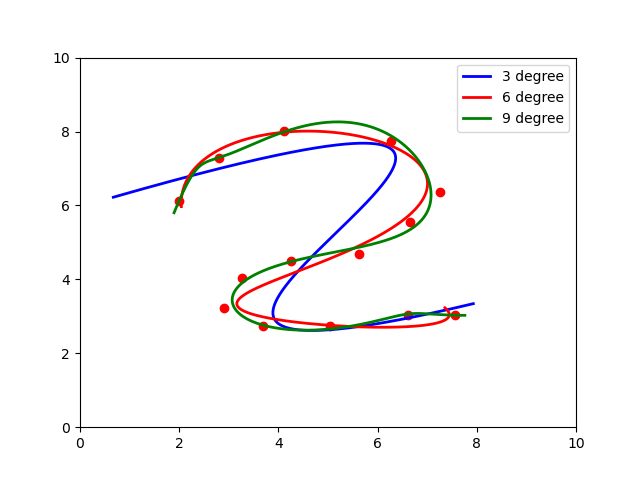
\includegraphics[width=5.5cm]{1.png}} %[图片大小]{图片路径}
    	\subfigure[]{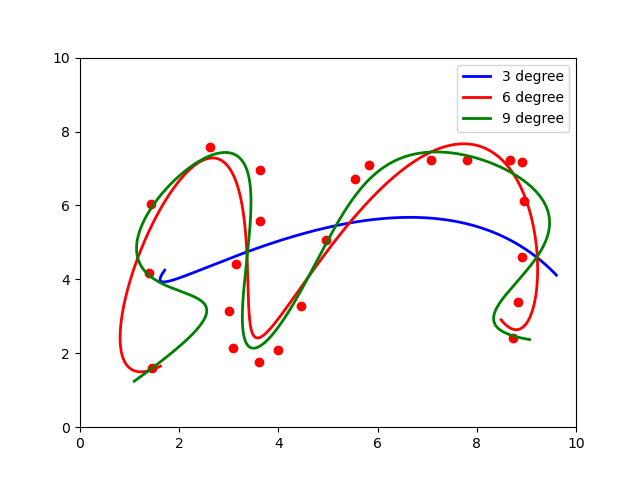
\includegraphics[width=5.5cm]{2.png}}
    	\subfigure[]{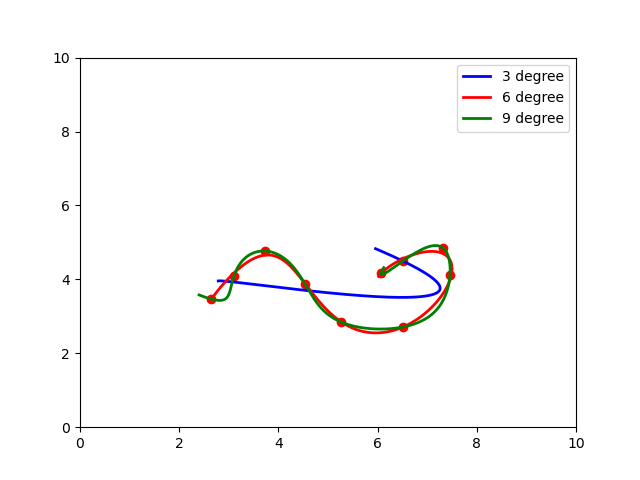
\includegraphics[width=5.5cm]{3.png}}
    	\caption{不同点列的3、6、9次多项式拟合} %图片标题
    	\label{fig:1}  %图片交叉引用时的标签
    \end{figure}
    
    \begin{figure}[htbp]
    	\centering %居中
    	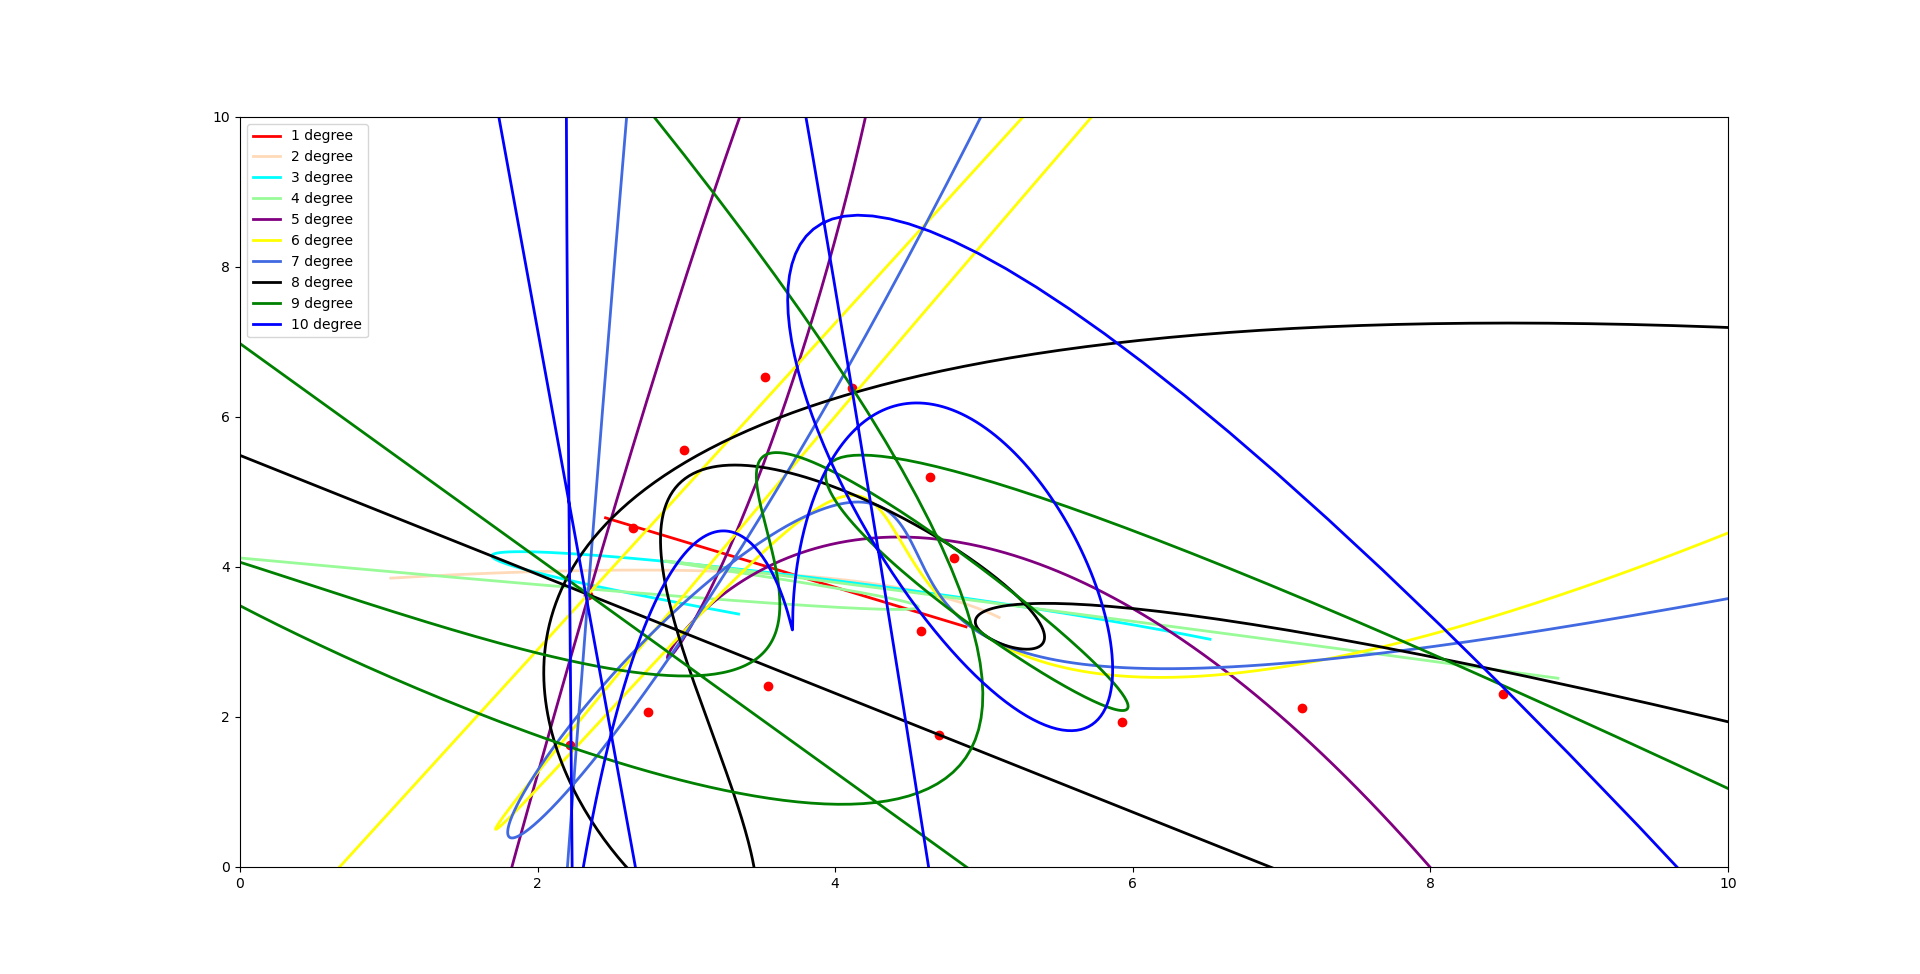
\includegraphics[scale=0.3]{tuya.png}
    	\caption{通过不同维度的多项式拟合得到的涂鸦}
    \end{figure}

	\begin{figure}[htbp]
		\centering
		\subfigure[] %子图片标题
		{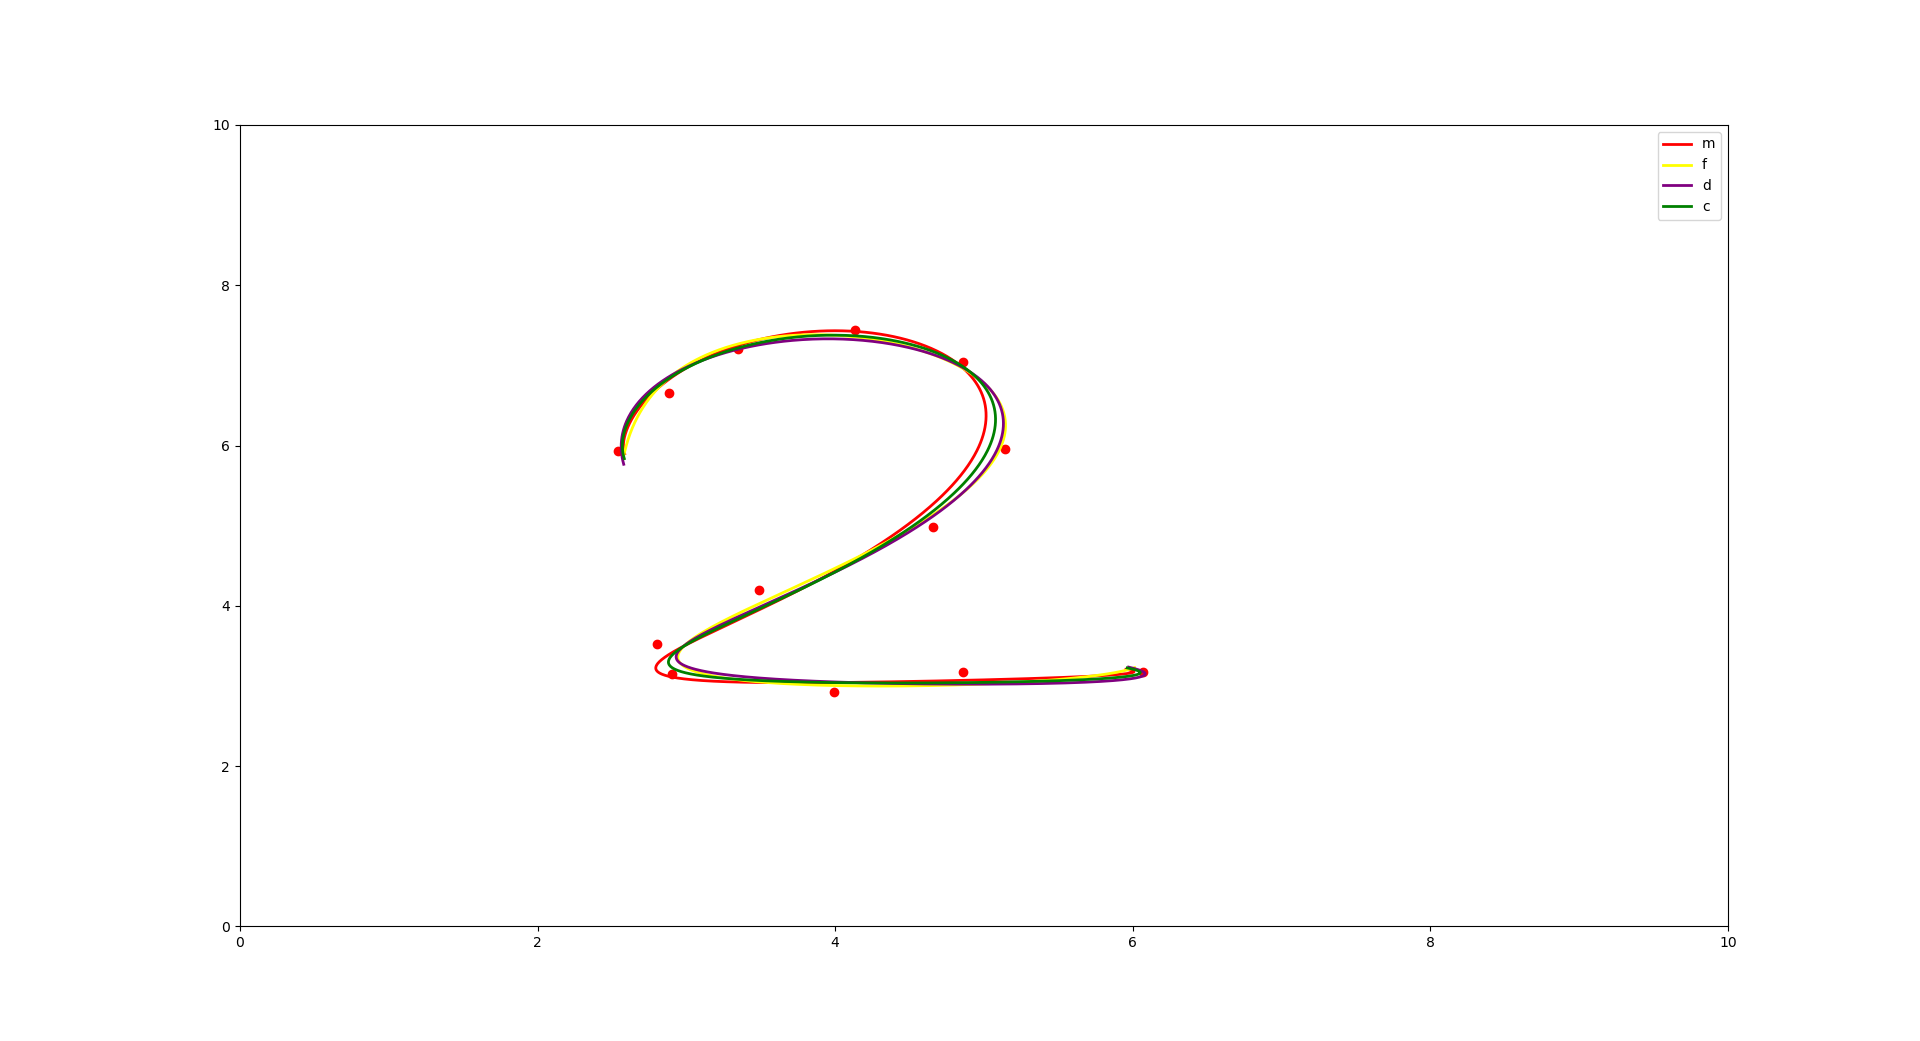
\includegraphics[width=5.5cm]{222.png}} %[图片大小]{图片路径}
		\subfigure[]{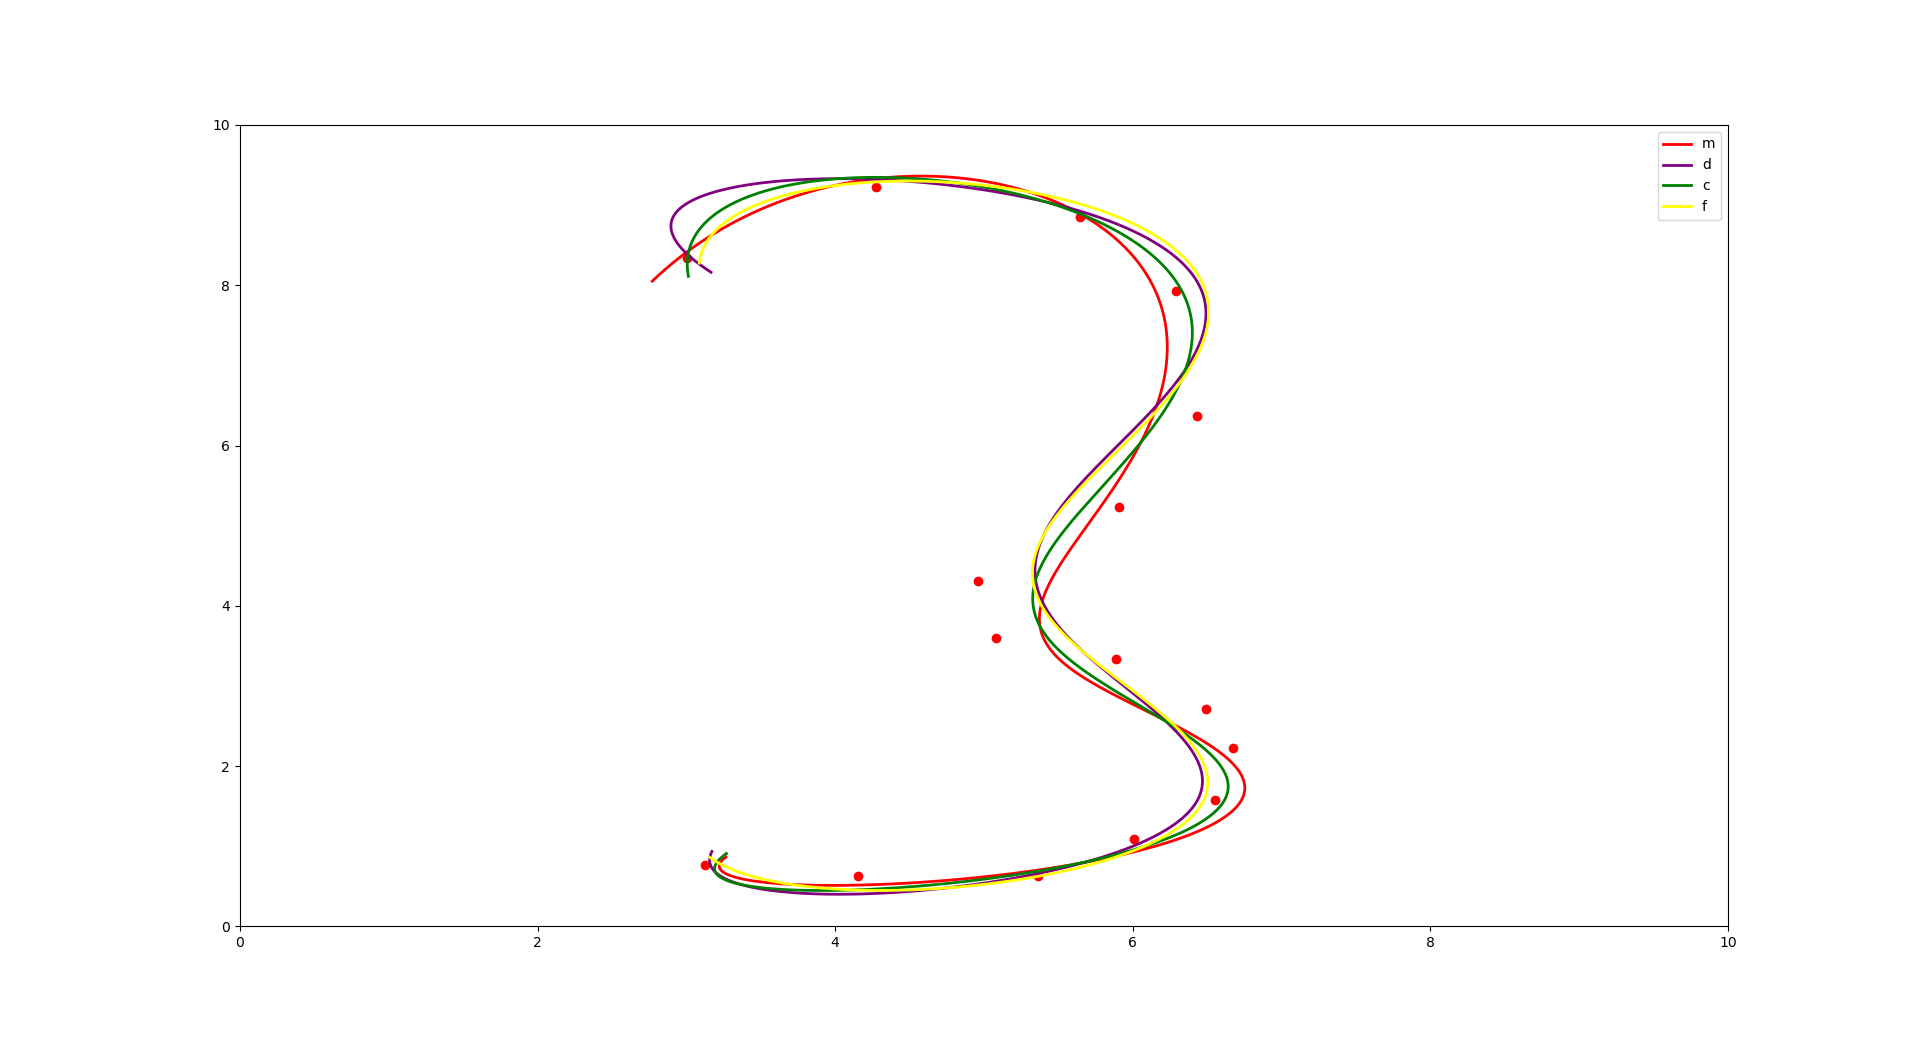
\includegraphics[width=5.5cm]{333.png}}
		\subfigure[]{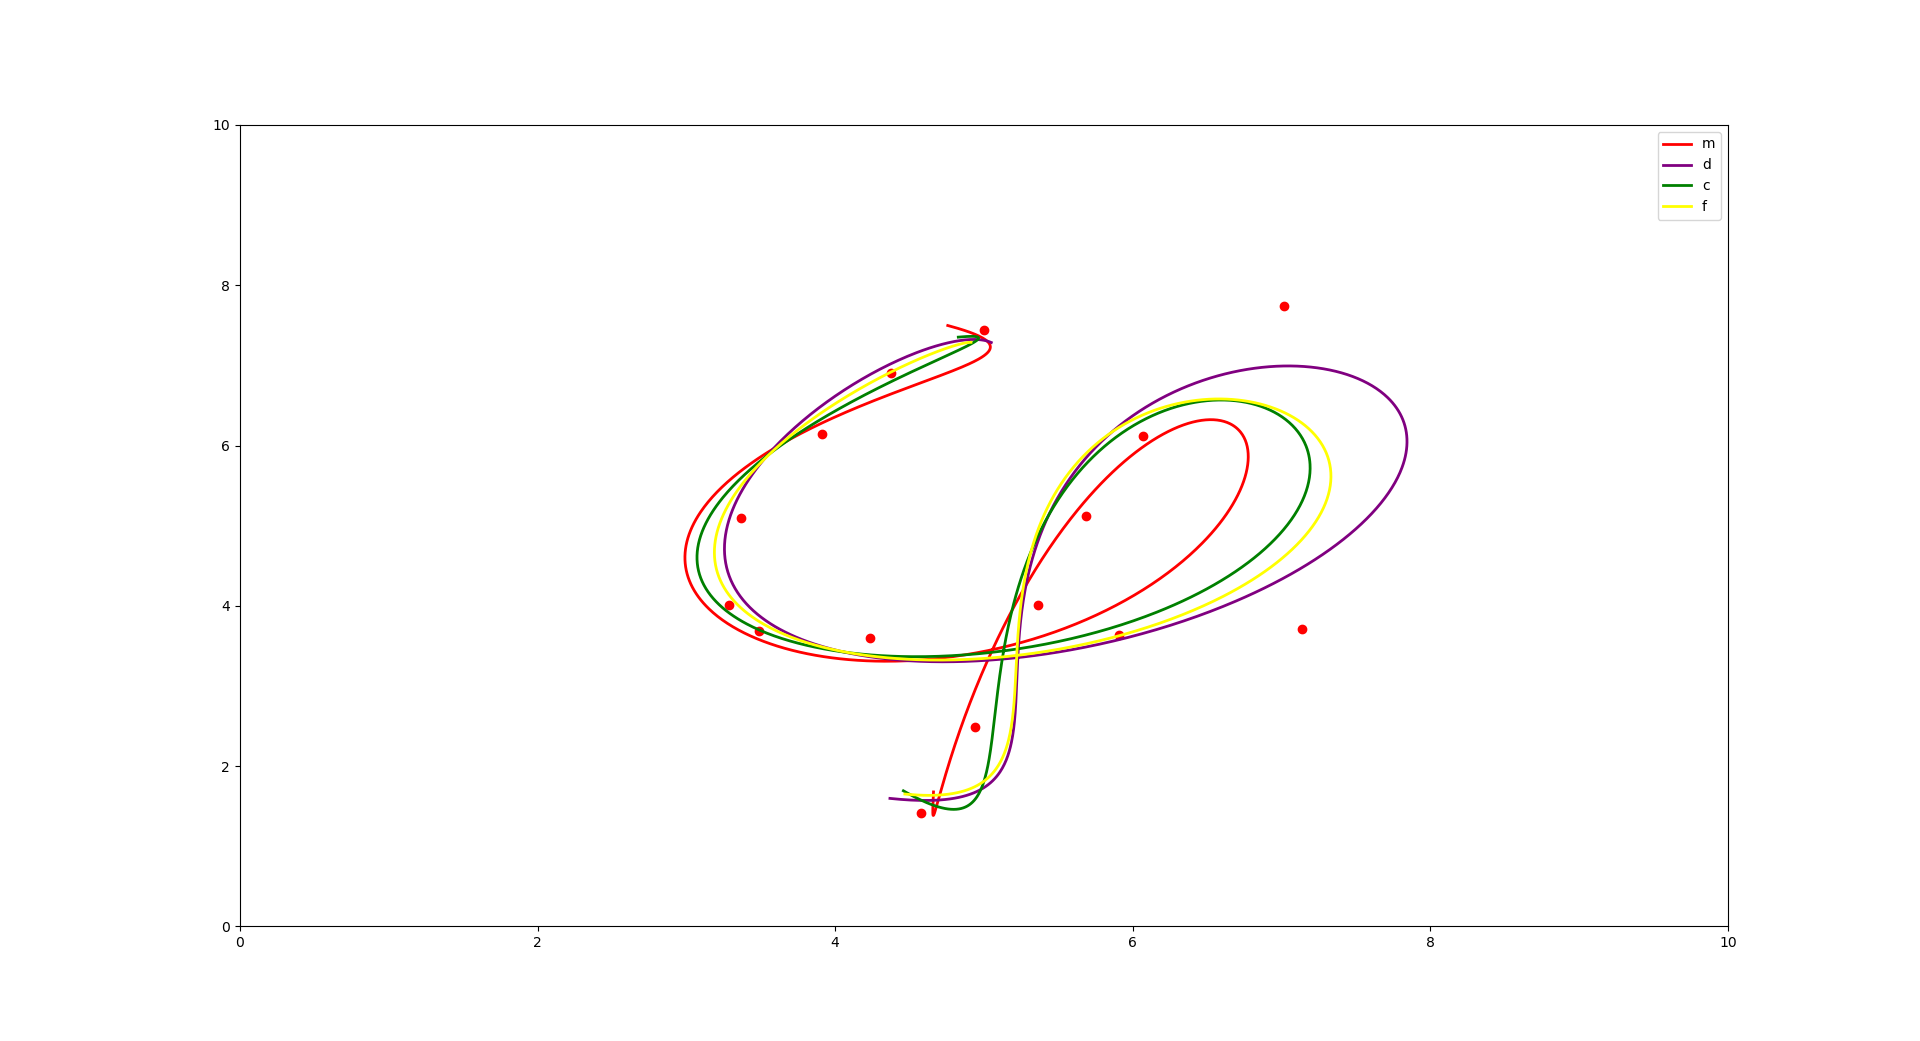
\includegraphics[width=5.5cm]{444.png}}
		\subfigure[] %子图片标题
		{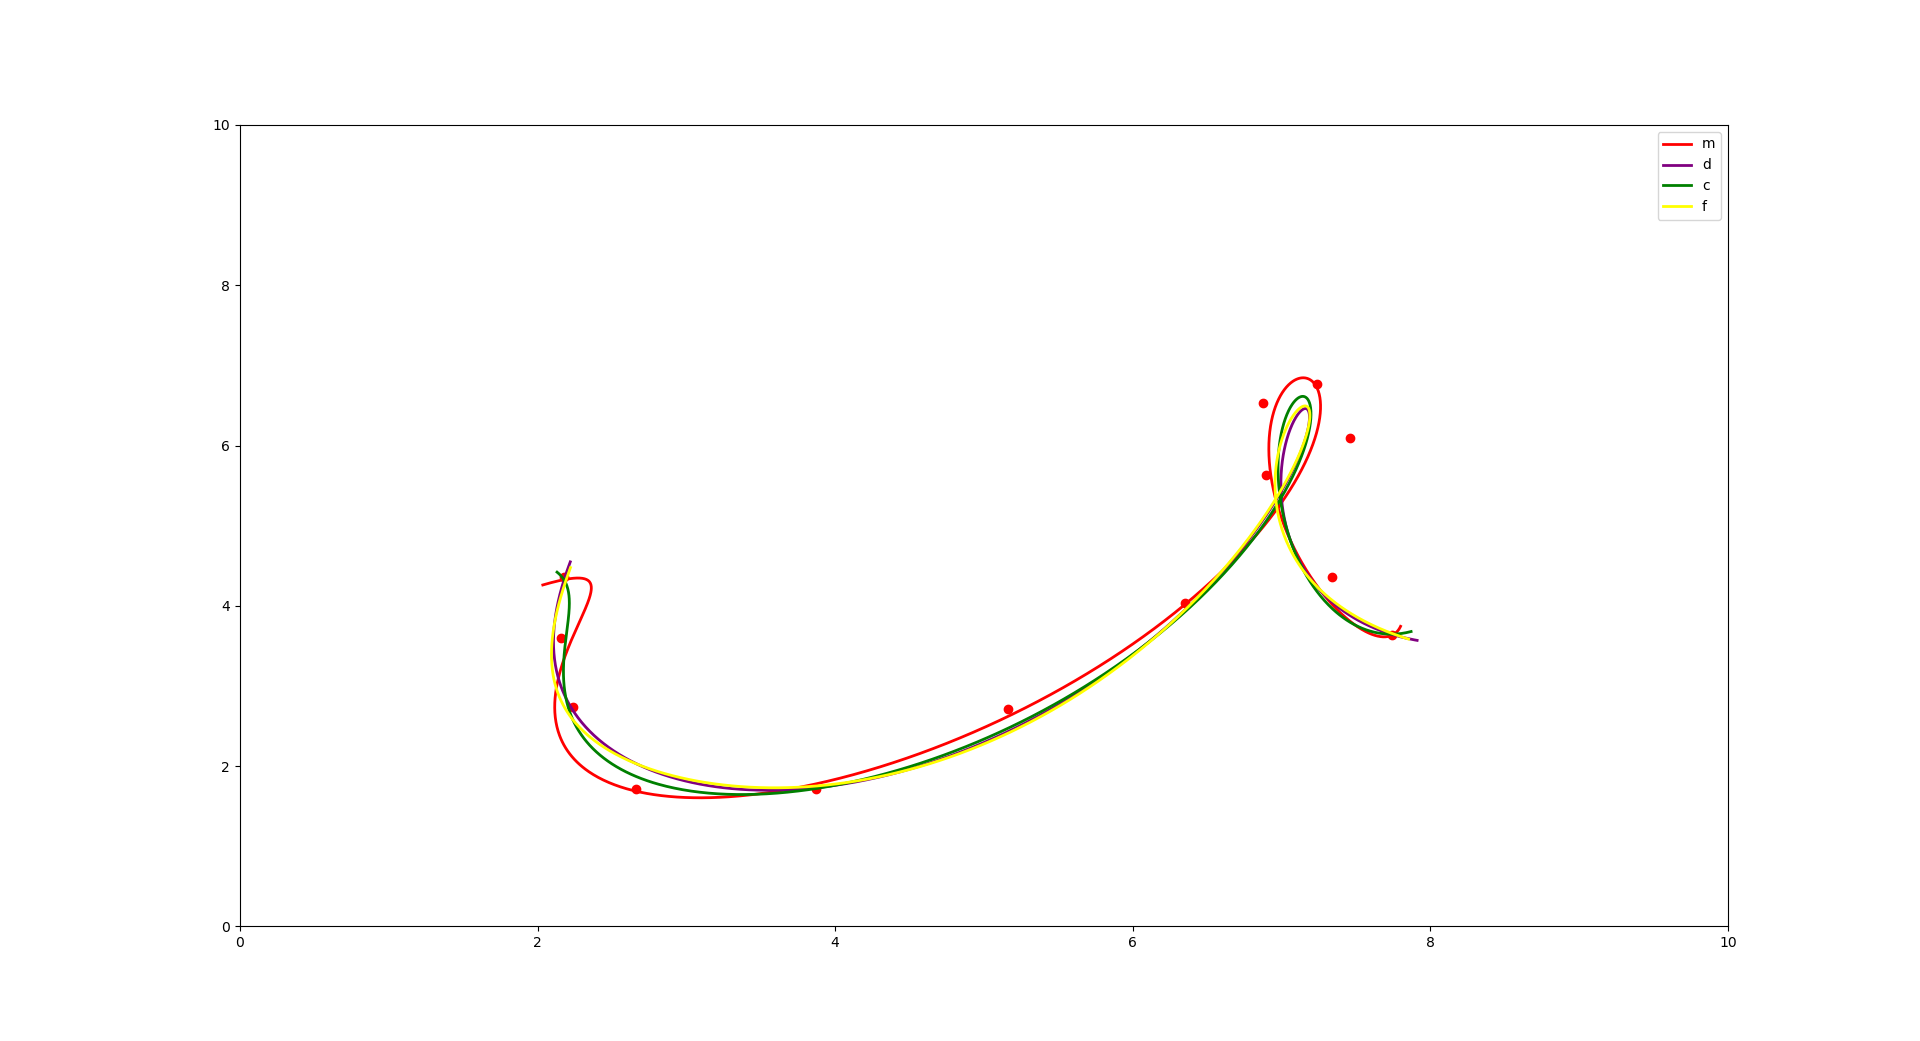
\includegraphics[width=5.5cm]{3d.png}} %[图片大小]{图片路径}
		\subfigure[]{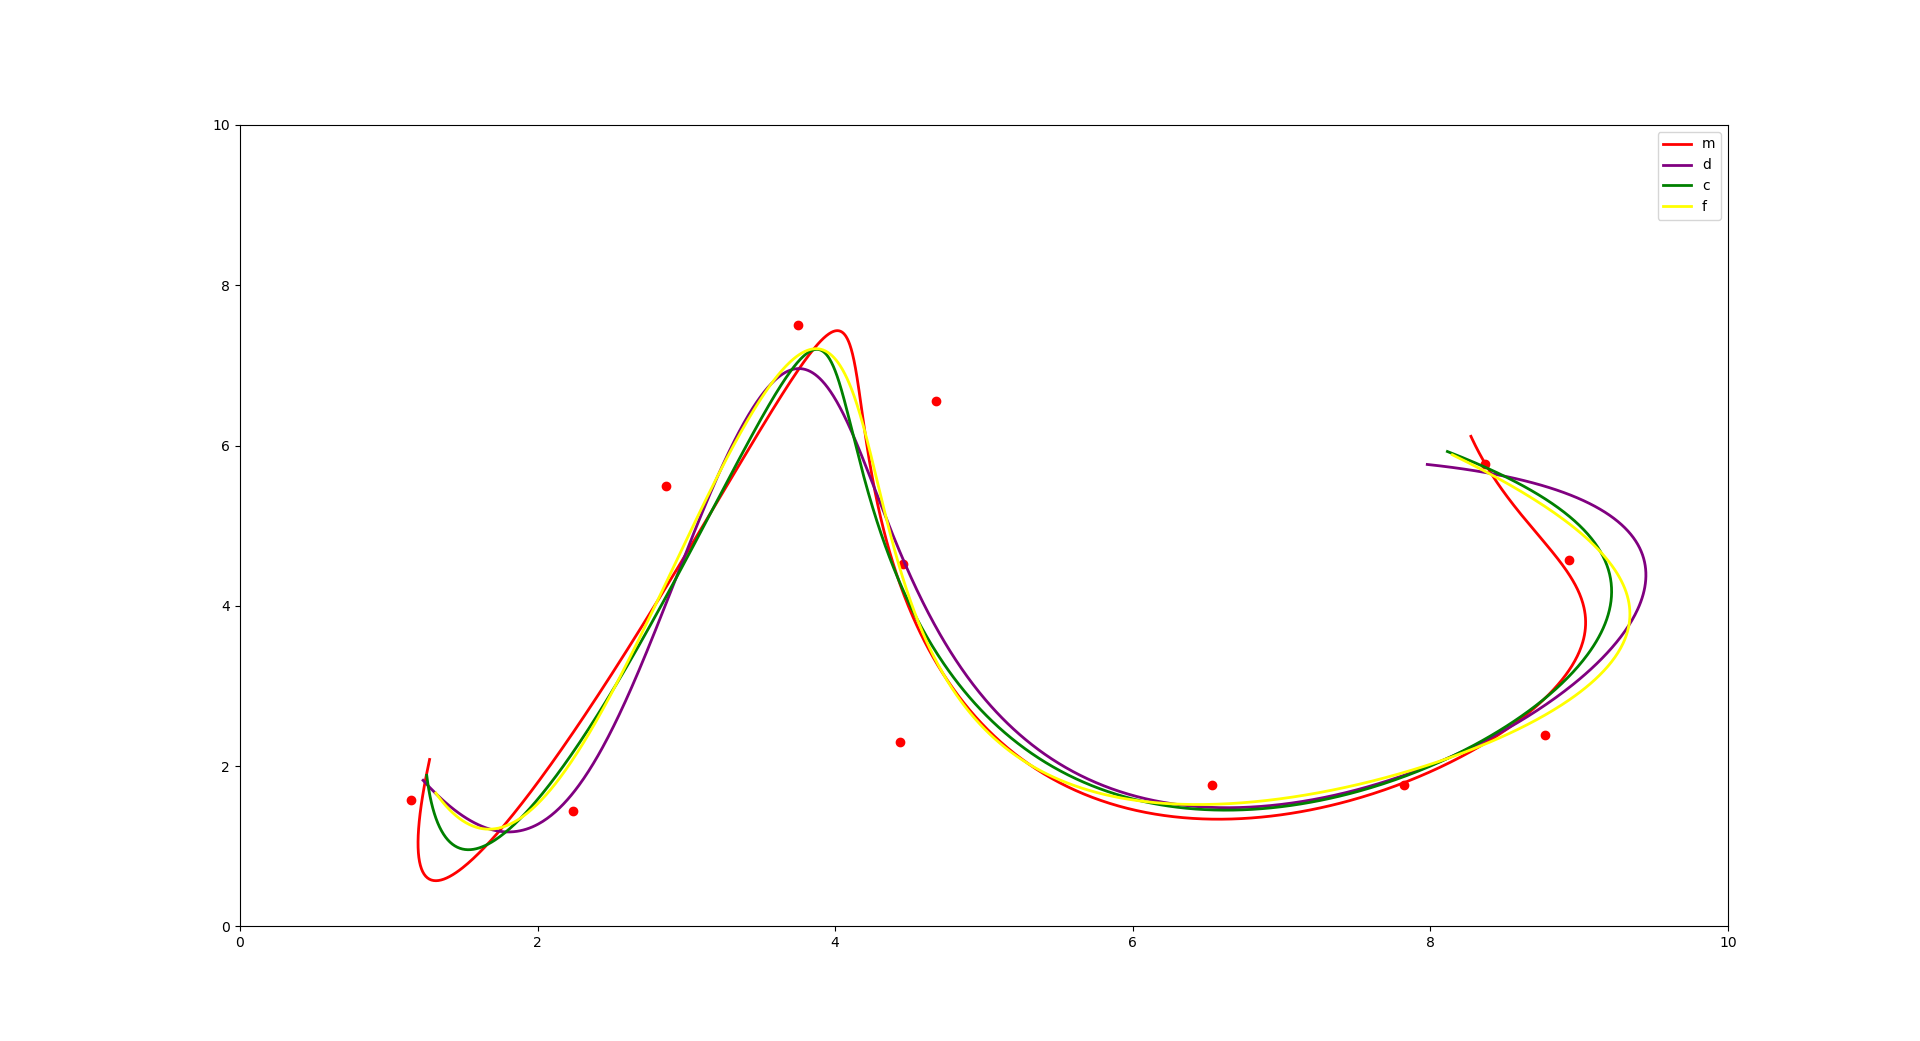
\includegraphics[width=5.5cm]{3e.png}}
		\subfigure[]{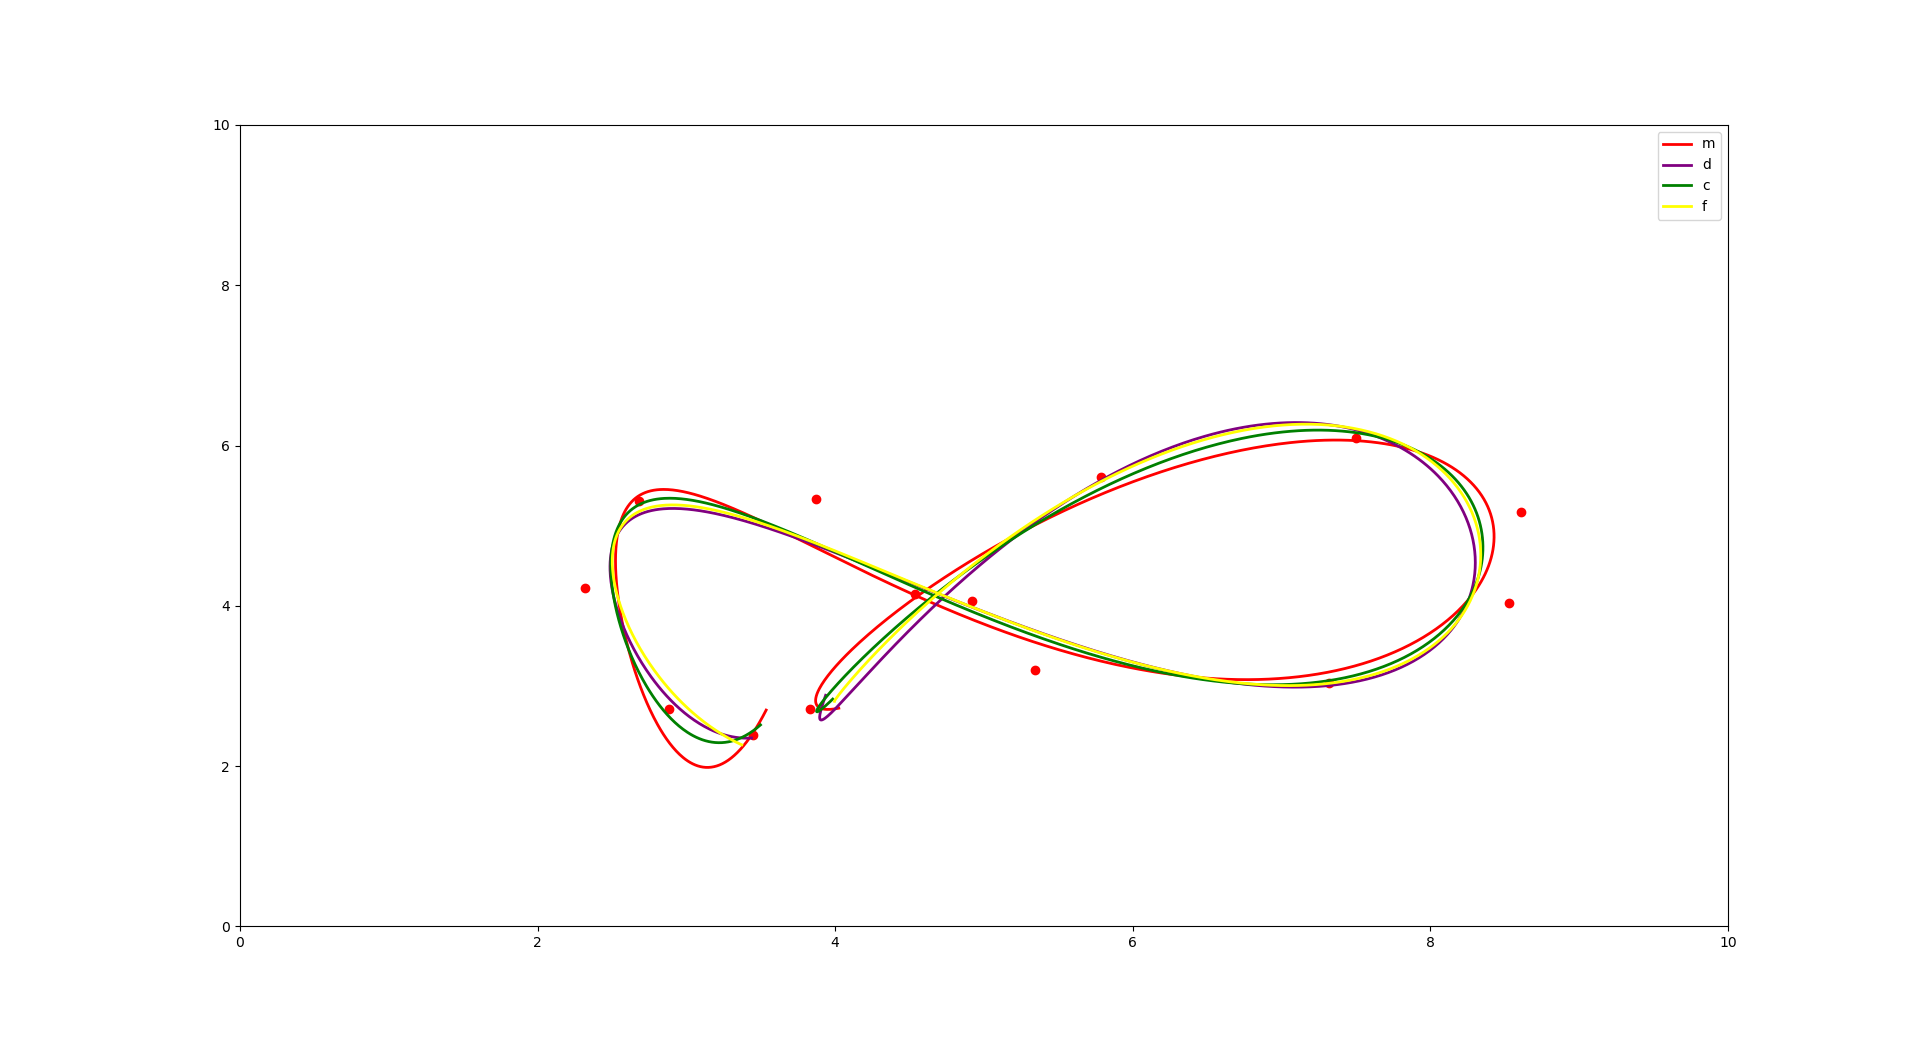
\includegraphics[width=5.5cm]{3f.png}}
		\caption{不同参数化法得到的拟合曲线} %图片标题
		\label{fig:1}  %图片交叉引用时的标签
	\end{figure}

	\begin{figure}[htbp]
		\centering
		\subfigure[] %子图片标题
		{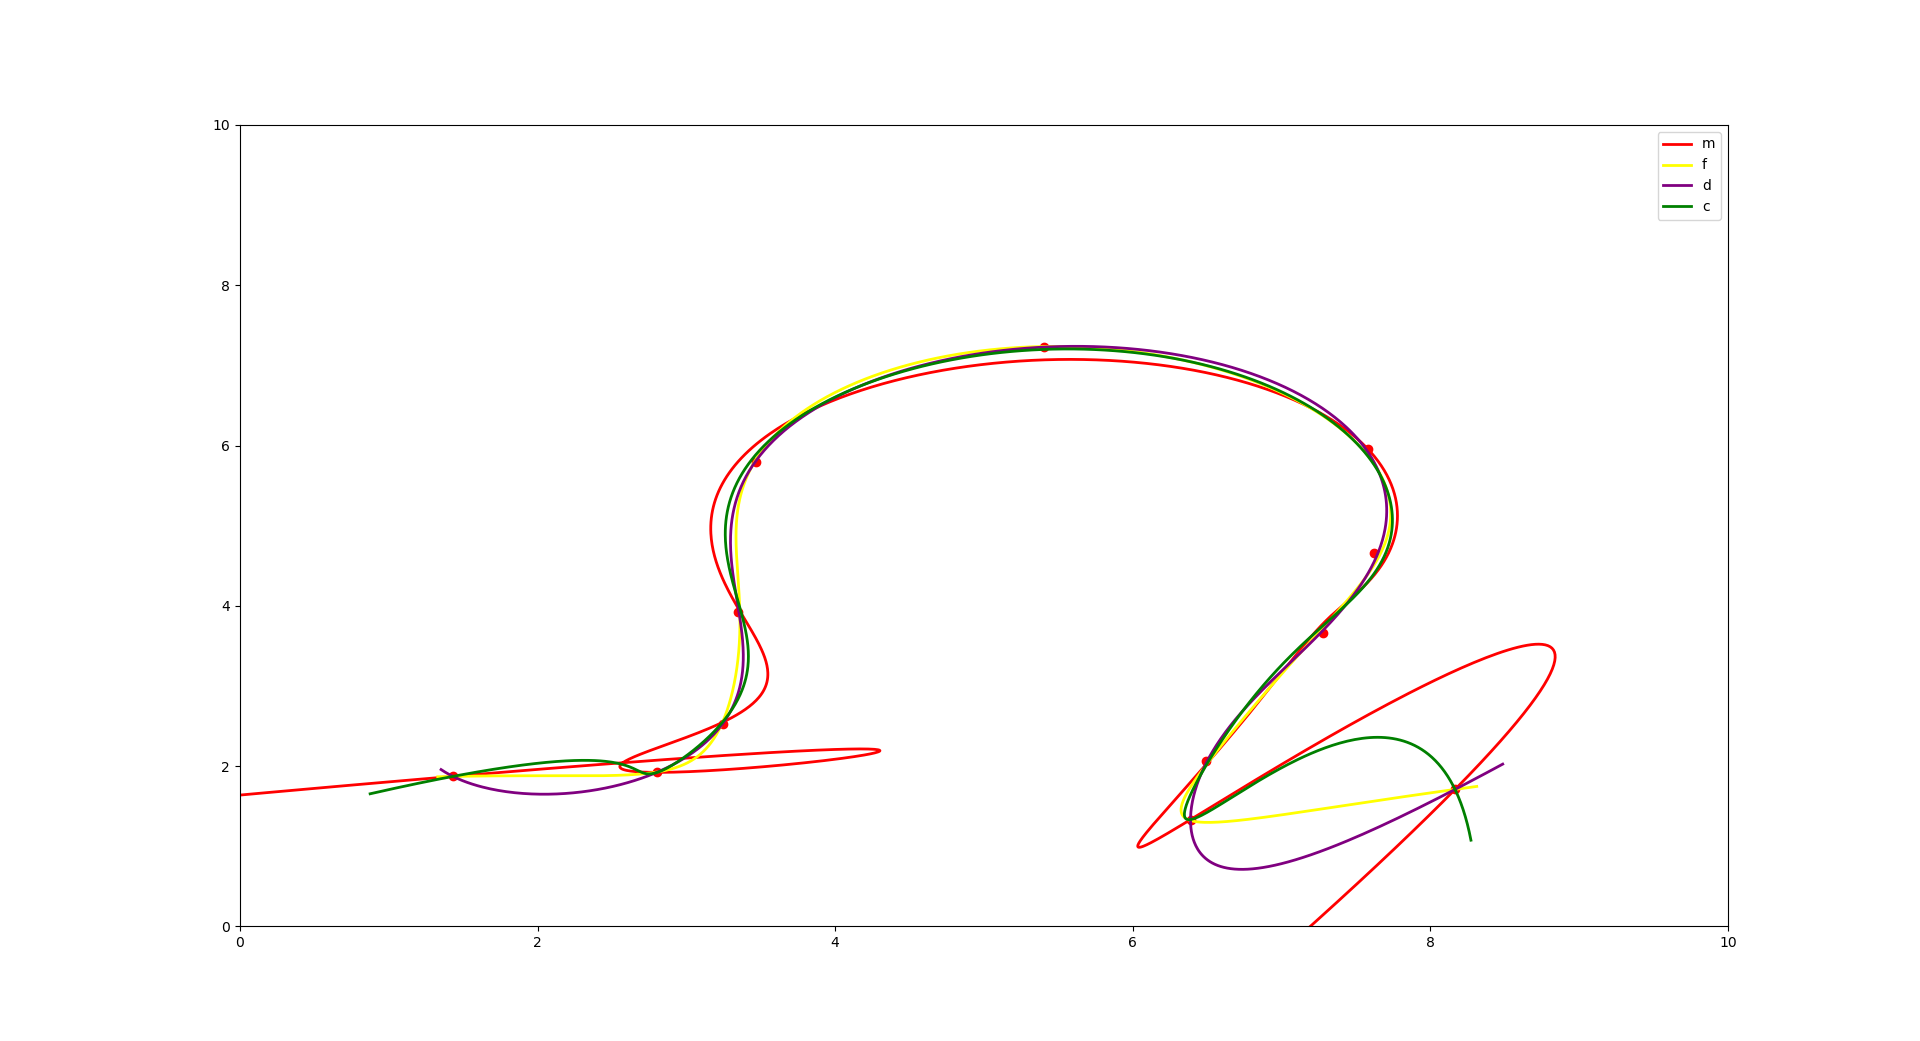
\includegraphics[width=8cm]{10mdcf.png}} %[图片大小]{图片路径}
		\subfigure[]{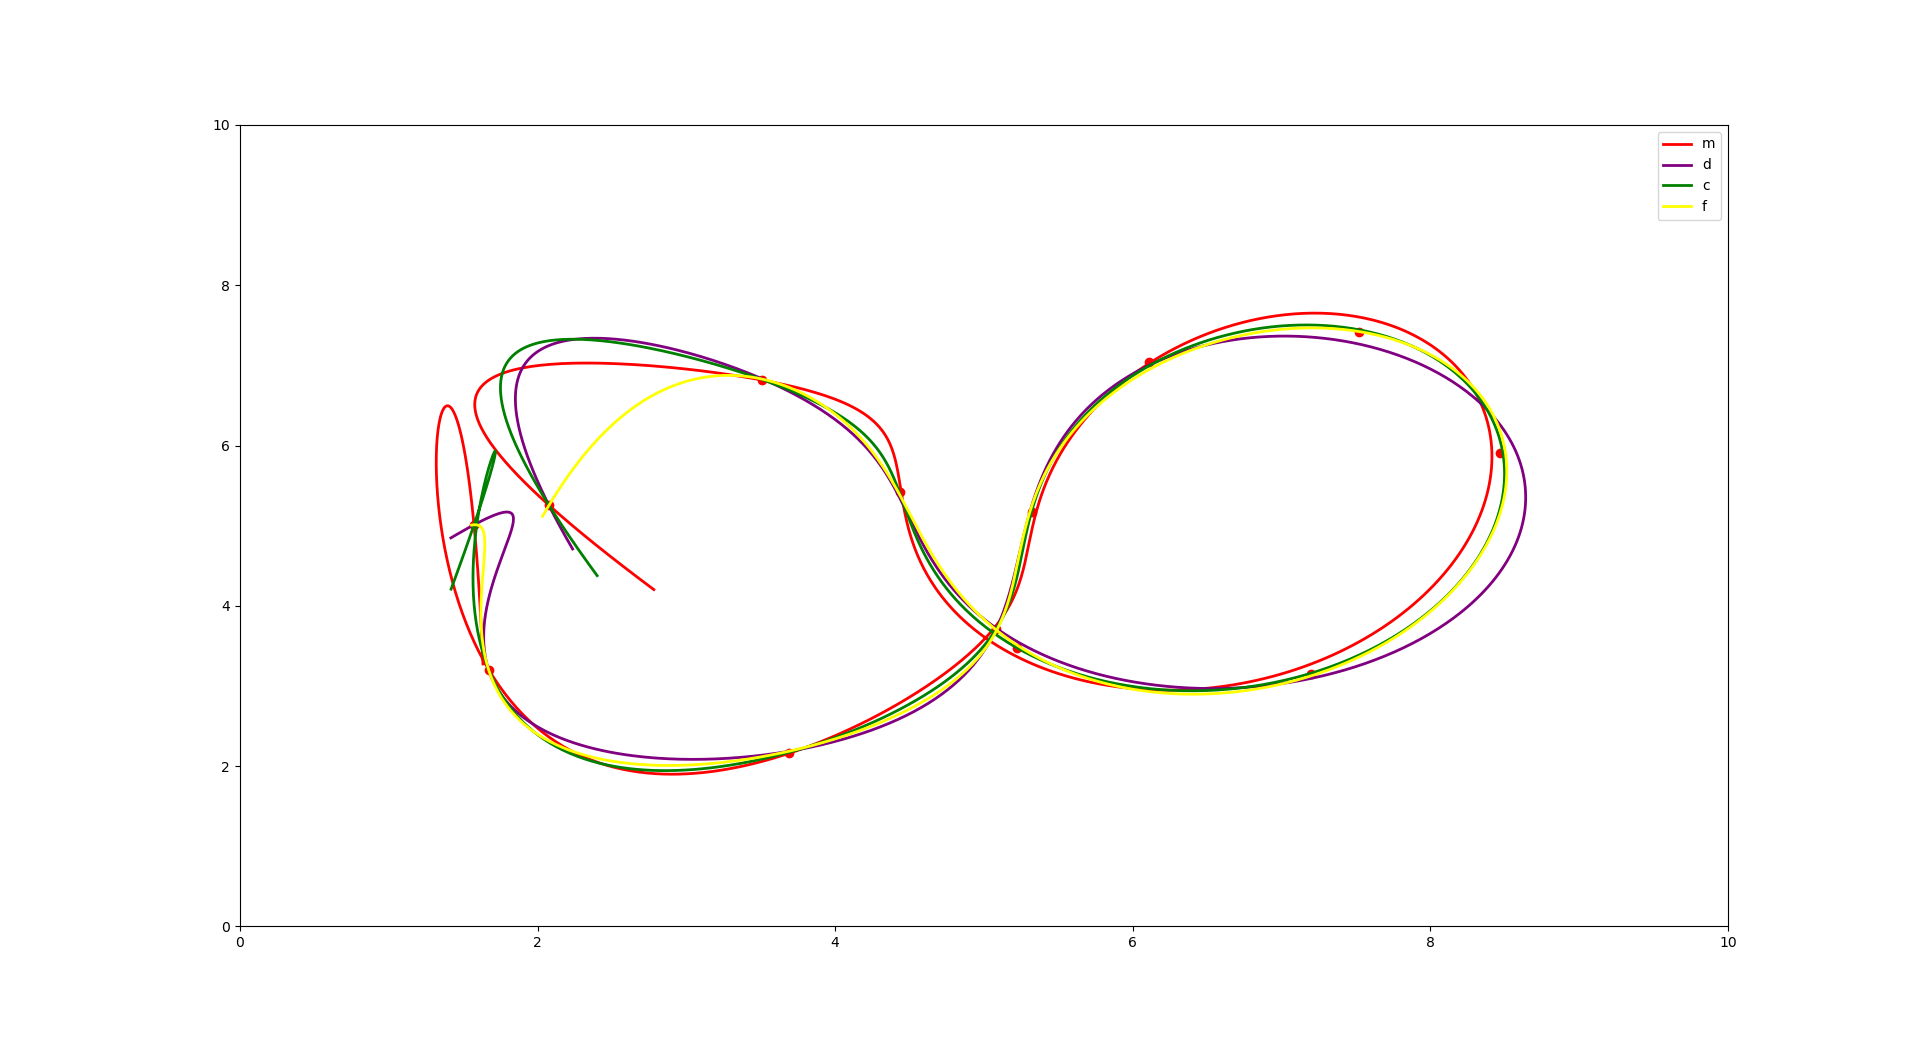
\includegraphics[width=8cm]{10mdcf2.png}}
		\caption{不同点列的3、6、9次多项式拟合} %图片标题
		\label{fig:1}  %图片交叉引用时的标签
	\end{figure}
	
	\begin{figure}[htbp]
		\centering
		\subfigure[控制点组1]{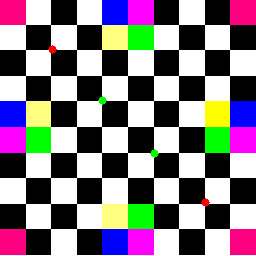
\includegraphics[width=2cm]{test1.png}} 
		\subfigure[IDW方法u=1]{\includegraphics[width=3cm]{Q_IDWU=1}}
		\subfigure[IDW方法u=2]{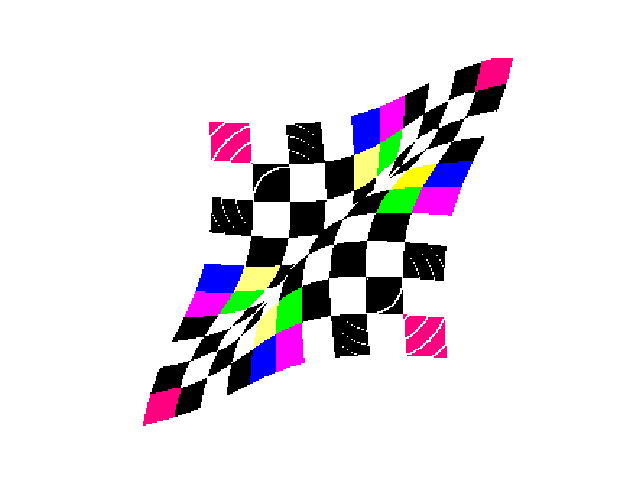
\includegraphics[width=3cm]{Q_IDWU=2}}
		\subfigure[IDW方法u=5]{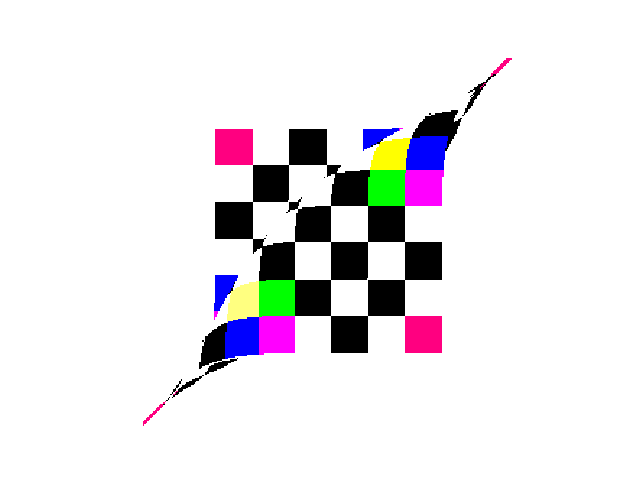
\includegraphics[width=3cm]{Q_IDWU=5}}
		\\ %换行
		\centering
		\subfigure[控制点组2]{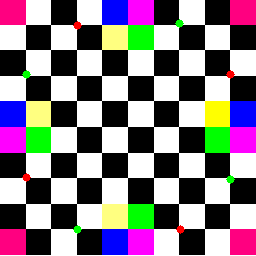
\includegraphics[width=2cm]{test2.png}} 
		\subfigure[IDW方法u=1]{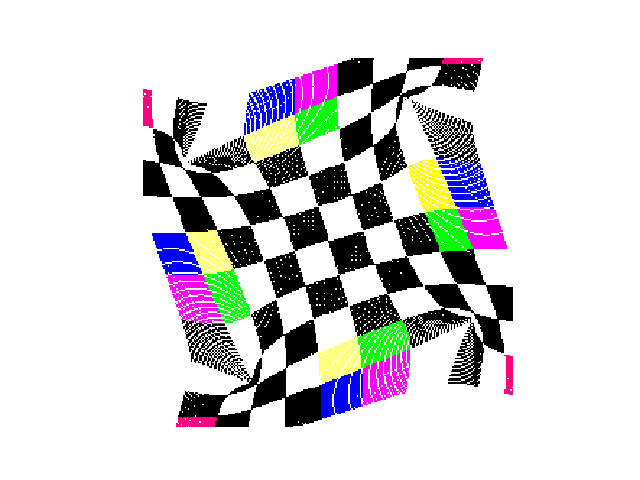
\includegraphics[width=3cm]{Q2_IDWU=1}}
		\subfigure[IDW方法u=2]{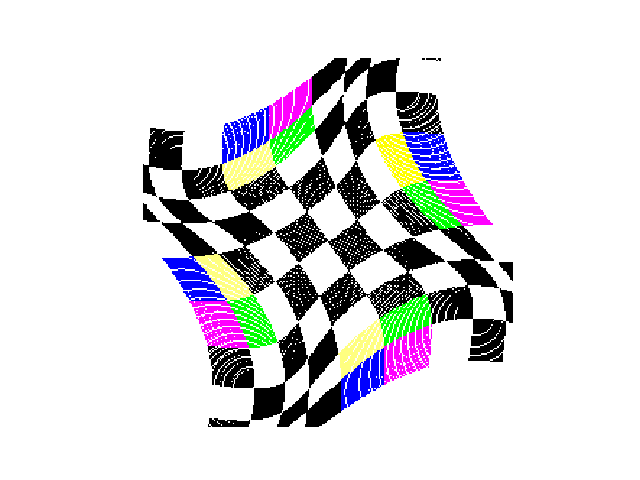
\includegraphics[width=3cm]{Q2_IDWU=2}}
		\subfigure[IDW方法u=5]{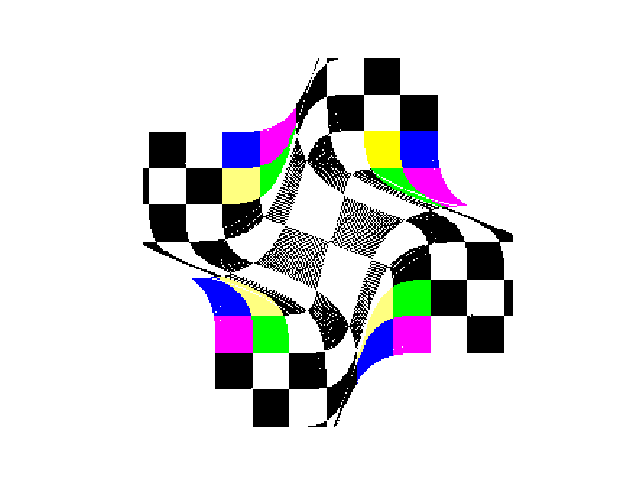
\includegraphics[width=3cm]{Q2_IDWU=5}}
		\caption{不同控制点及不同u取值的IDW方法比较} %图片标题
	\end{figure}

	\begin{figure}[htbp]
		\centering
		\subfigure[控制点组1]{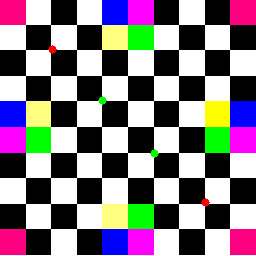
\includegraphics[width=2.5cm]{test1.png}} 
		\subfigure[RBF方法u=1]{\includegraphics[width=4cm]{Q_RBFU=1}}
		\subfigure[RBF方法u=5]{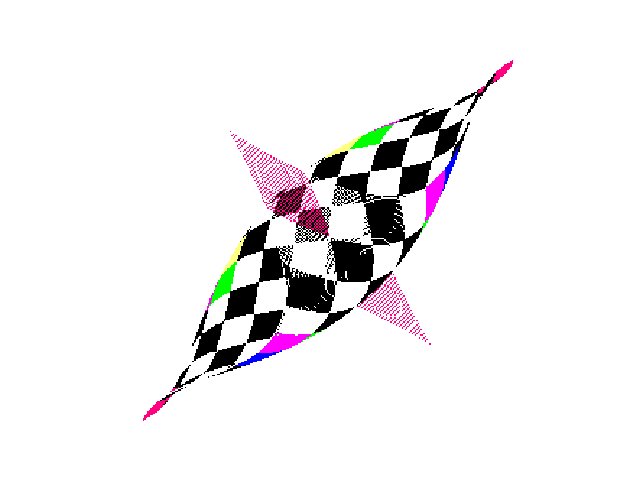
\includegraphics[width=4cm]{Q_RBFU=5}}
		\\ %换行
		\centering
		\subfigure[控制点组2]{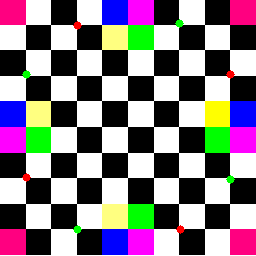
\includegraphics[width=2.5cm]{test2.png}} 
		\subfigure[RBF方法u=1]{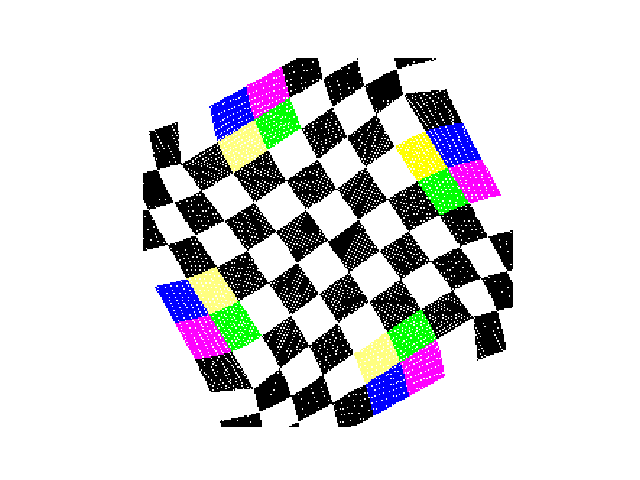
\includegraphics[width=4cm]{Q2_RBFU=1}}
		\subfigure[RBF方法u=5]{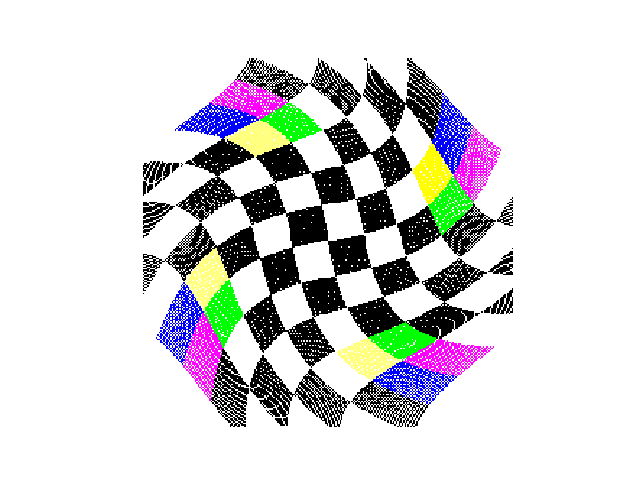
\includegraphics[width=4cm]{Q2_RBFU=5}}
		\caption{不同控制点及不同u取值的RBF方法比较} %图片标题
	\end{figure}

	\begin{figure}[htbp]
		\centering
		\subfigure[原图] %子图片标题
		{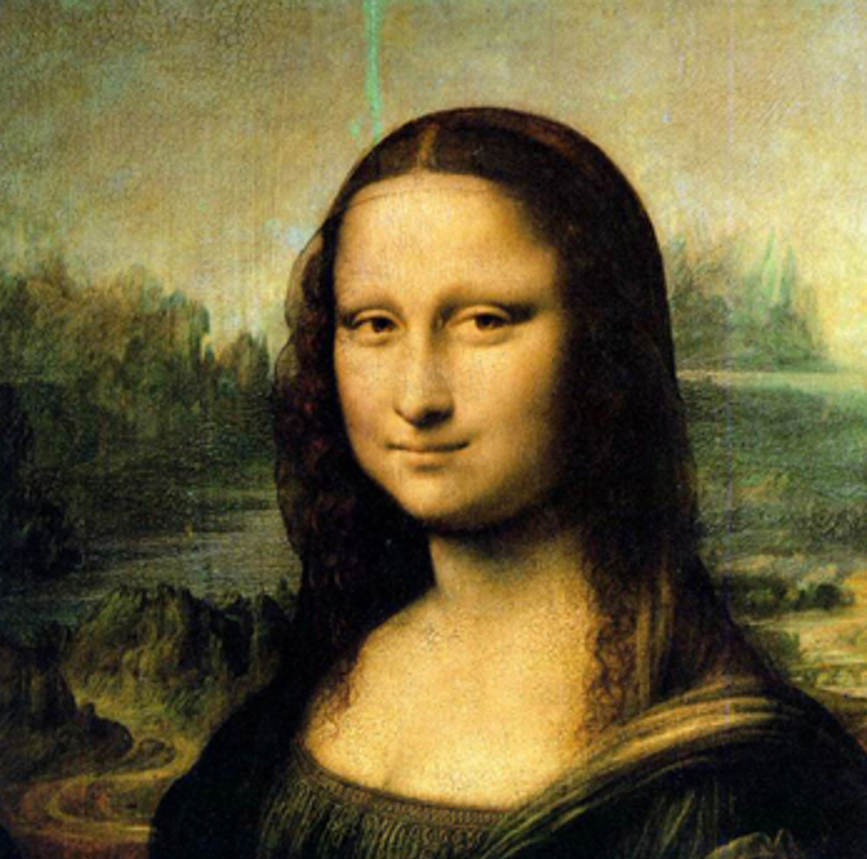
\includegraphics[width=3.8cm]{Monalisa.png}} %[图片大小]{图片路径}
		\subfigure[IDW方法(u=2)]{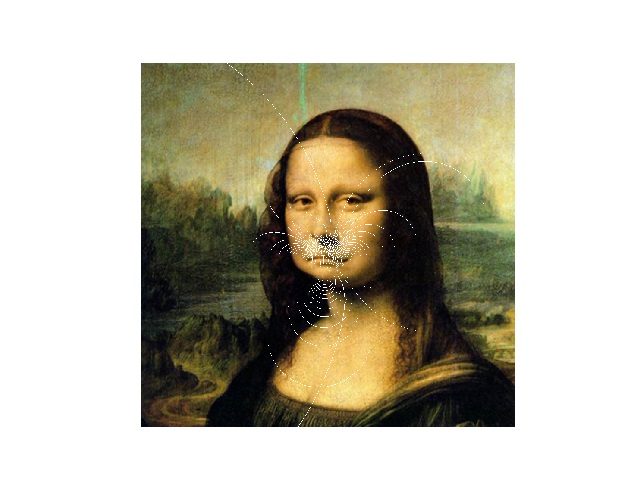
\includegraphics[width=5.5cm]{uncolorIDW.png}}
		\subfigure[RBF方法(u=1)]{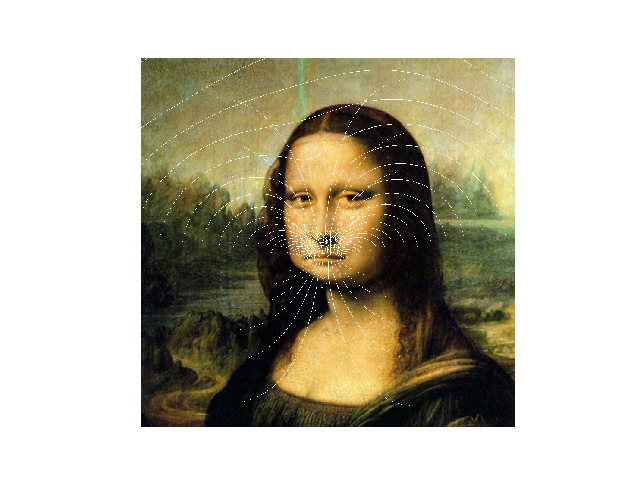
\includegraphics[width=5.3cm]{uncolorRBF.png}}
		\caption{“蒙娜丽莎的苦脸”} %图片标题
		\label{fig:1}  %图片交叉引用时的标签
	\end{figure}


	\begin{figure}[htbp]
		\centering
		\subfigure[原图] %子图片标题
		{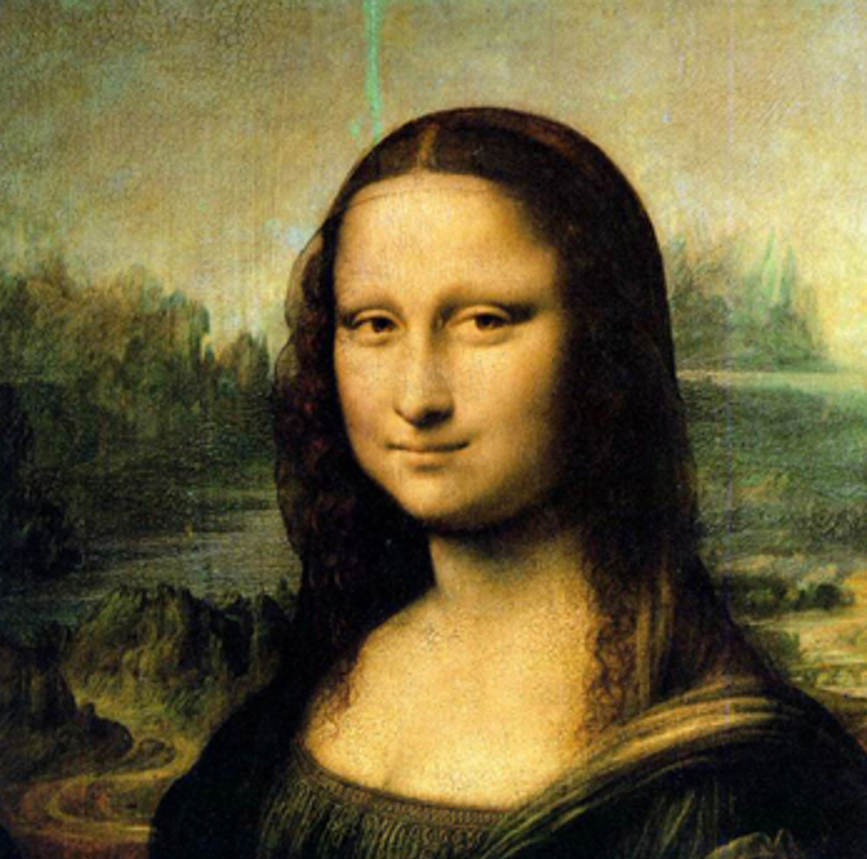
\includegraphics[width=3.8cm]{Monalisa.png}} %[图片大小]{图片路径}
		\subfigure[IDW方法(u=2)]{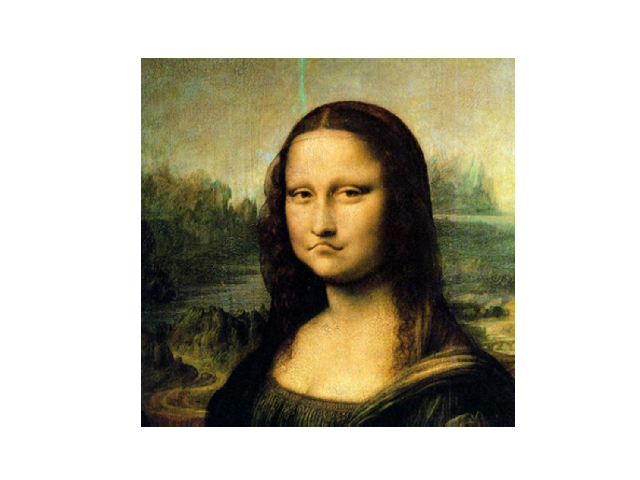
\includegraphics[width=5.5cm]{M_1.png}}
		\subfigure[RBF方法(u=1)]{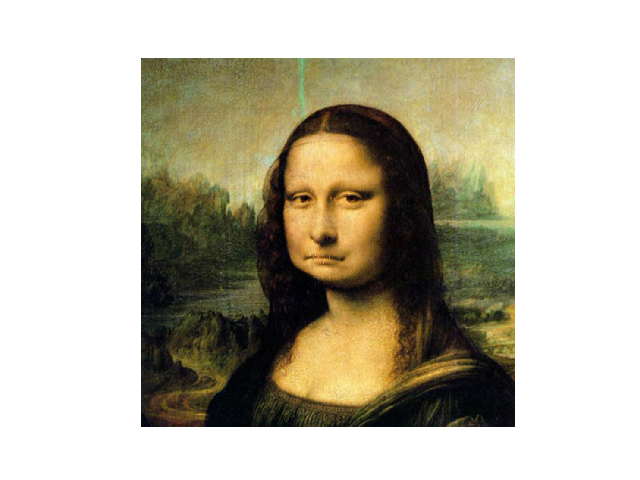
\includegraphics[width=5.3cm]{M1_RBF.png}}
		\caption{“蒙娜丽莎的苦脸”} %图片标题
		\label{fig:1}  %图片交叉引用时的标签
	\end{figure}

	\begin{figure}[htbp]
		\centering
		\subfigure[原图] %子图片标题
		{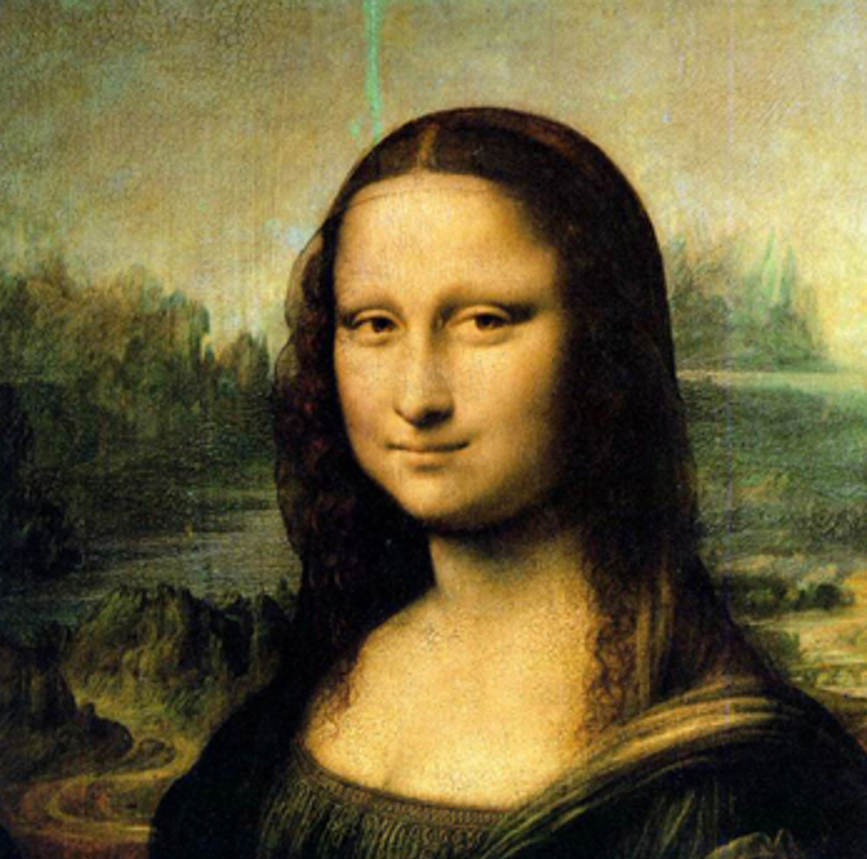
\includegraphics[width=3.8cm]{Monalisa.png}} %[图片大小]{图片路径}
		\subfigure[IDW方法(u=2)]{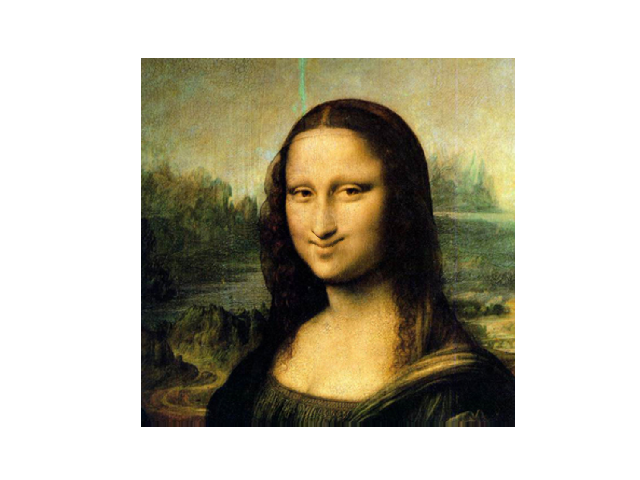
\includegraphics[width=5.5cm]{M_2.png}}
		\subfigure[RBF方法(u=1)]{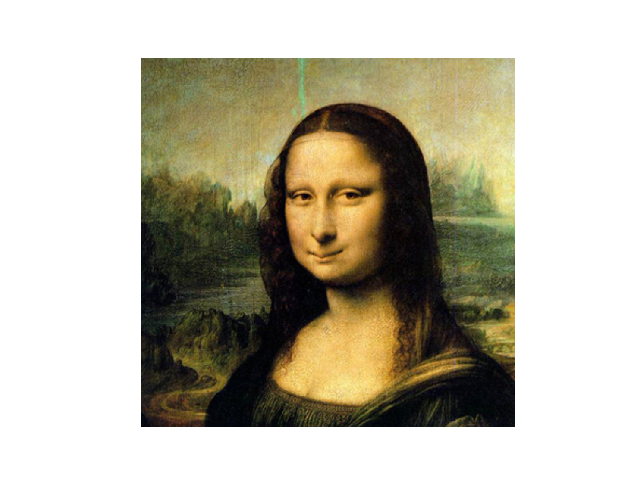
\includegraphics[width=5.3cm]{M2_RBF.png}}
		\caption{“蒙娜丽莎的大笑”} %图片标题
		\label{fig:1}  %图片交叉引用时的标签
	\end{figure}


 \setcounter{section}{8}
\section*{\centerline{八、问题与优化}}
    \begin{itemize}
    	\item [1)]
    	IDW算法与RBF算法中得到的映射会映射成一对小数坐标,而计算机的图片存储的坐标都是整数,所以计算过程中要进行取整操作。
    	\item [2)]
    	填色过程中可以取该点周围8个点的平均值这样能使图片更加平滑。
    	\item [3)] 
    	进行Foley-Nielsen参数化时容易出现边界值越界的问题,所以要在程序中做好边界值的处理,对$i=0,i=n$两处进行特别处理。
    	\item [4)]
    	高次多项式回归会造成过拟合,可以通过正则化的方式来对高次系数进行惩罚,得到更好的拟合效果。
    \end{itemize}  

 \setcounter{section}{9}
\section*{\centerline{九、代码及程序说明}}
	具体代码见压缩包中的三个py文件。
	
	其中degreeCompare.py文件为比较不同维度多项式回归结果的程序代码,默认使用弦长参数化法,可在程序中自主调节。选点后,按1~9中任意数即可得到该数维度的多项式回归的结果,按其他按键会按十次多项式回归得到曲线。
	
	parameterizationCompare.py为比较不同参数化方法的程序代码,可改变全局变量exp设置回归多项式次数,默认为十次。鼠标选点后按'm','d','c','f'分别代表进行均匀参数化、弦长参数化、中心参数化、福利参数化,默认使用福利参数化。
	
	imageWraping.py为图形变换代码,运行后鼠标按下点为控制起点,松开点为控制终点,控制点选好后按'i'为使用IDW方法,其他键为使用RBF方法。可以改变全局变量改变u的值进行测试,也可以改变imageName全局变量用不同的图进行测试 
	
\clearpage
\bibliographystyle{ieeetr}
\bibliography{refer}

\end{document}